\chapter{Számformátumok}
\thispagestyle{empty}

\section{Százalék és pénznem formátum}

A számokat tartalmazó cellákon speciális formázásokat
állíthatunk be. A leggyakrabban használt számformátumok az
eszköztáron is elérhetők: százalék és a pénznem
formátum. E két alapvető formátum megértéséhez írjuk
be a következő adatokat (\ref{Számformátumok} ábra).

\begin{figure}[!h]
\begin{center}
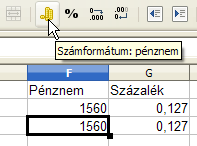
\includegraphics[width=5.211cm]{oocalcv1-img42.png}
\caption{Számformátumok}\label{Számformátumok}
\end{center}
\end{figure}

Az F3 cellán állítsunk be pénznem-, a G3 cellán pedig
százalékformátumot. Látjuk \aref{SzázalékFormátum} ábrán, hogy a pénznem
formátum ezres csoportosítást, két tizedesjegynyi pontosságot
állított be és hozzáadta az alapértelmezett pénznem
megjelölést. A százalék formátum a számot százzal
megszorozva, két tizedesjegynyi pontossággal és a
százalékjellel kiegészítve mutatja.

\begin{figure}[!h]
\begin{center}
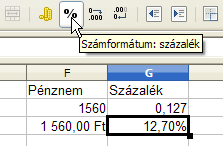
\includegraphics[width=5.898cm]{oocalcv1-img43.png}
\caption{Százalék formátum}\label{SzázalékFormátum}
\end{center}
\end{figure}

A tizedesjegyek számát növelhetjük és csökkenthetjük a
\textbf{Formátum} eszköztár \textbf{Számformátum: tizedesjegy
hozzáadása} és a \textbf{Számformátum: Tizedesjegy
törlése} kapcsolókkal. A Calc a matematika szabályai szerint
kerekít a tizedesjegyek számának csökkentésekor, de vegyük
figyelembe, hogy ilyenkor a cellában kerekítve látjuk a
számértéket, de a cella tartalma közben nem változik.
Esetünkben, ha nullára csökkentjük a tizedesjegyek számát a
G3 cellában, abban 13\%-ot fogunk látni, de a cella tartalma
továbbra is 0,127 marad.

A százalékformátum ilyen megvalósítása megkönnyíti a
százalékszámításokat: pl. az A1 cellába írt szám B1
cellába felvett százalékát a két cella szorzatával
számíthatjuk ki.

A \textbf{Formátum} eszköztár \textbf{Számformátum:
Általános} kapcsolóval törölhetjük a számformátumokat a
kijelölt cellákon, és a cella ismét alapértelmezett
számformátumú lesz.


\section{9. feladat}
{\itshape
Egy üzlet 20 db péksütemény vásárlásakor 5\%, 50 db
esetén 8\% kedvezményt ad. Számítsuk ki a kedvezményes
árakat a D2:D6 és az E2:E6 tartományokban a D10, D11 cellákban
felvett százalékértékekkel számolva (\ref{9-feladat} ábra).}

{\itshape
Az F oszlopban számítsuk ki egy kilogramm péksütemény árát
az eredeti áron számolva. Ezekből az árakból határozzuk
meg, hogy hány százalékkal drágább a fonott kalács mint a
zsemle.}

{\itshape
A táblázatot a calc02 munkafüzet harmadik munkalapján hozzuk
létre, amelyiket nevezzünk át Kedvezmény-re.}

\begin{figure}[!h]
\begin{center}
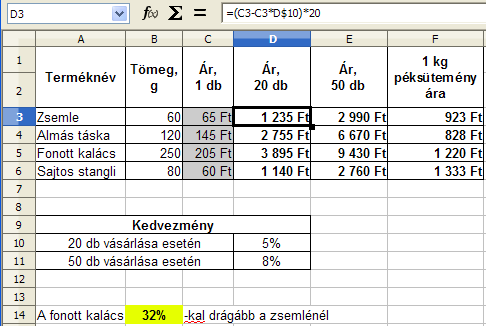
\includegraphics[width=12.857cm]{oocalcv1-img44.png}
\caption{9. feladat}\label{9-feladat}
\end{center}
\end{figure}

\Aref{9-feladat} ábrán figyeljük meg a D3 cella tartalmát:
\textsf{\textbf{=(C3-C3*D\$10)*20}}. Az eredeti árból (C3) kivonjuk
a kedvezményt, amit az eredeti ár és a kedvezmény szorzatával
(C3*D\$10) határozunk meg. Ne feledjük, hogy a D10 cella
számértéke 0,05.

A képletben zárójelből kiemelve a C3-at a következő
kifejezést kapjuk  \textsf{\textbf{=20*C3*(1-D\$10)}}.

Az E3 cellát ezzel a módszerrel számítsuk ki (\ref{9-feladatE3} ábra).

\begin{figure}[!h]
\begin{center}
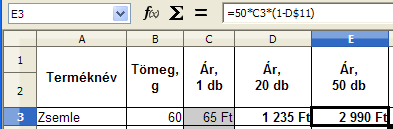
\includegraphics[width=10.396cm]{oocalcv1-img45.png}
\caption{9. feladat}\label{9-feladatE3}
\end{center}
\end{figure}

Az F oszlopban egy kilogramm péksütemény árát a
\textsf{\textbf{=}}\textsf{\textbf{B3/C3*1000}} képlettel
számíthatjuk ki, hiszen a B3/C3 egy gramm árát adja meg.

Azt, hogy hány százalékkal több az F5 mint az F3, egy tört
adja meg, aminek számlálója a két cella különbsége,
nevezője pedig az F3. A B14 cella tartalma tehát:
\textsf{\textbf{=(F5-F3)/F3}}, számformátuma százalék,
tizedeshelyek száma nulla.


\section{Dátum- és időformátum}

A Calc a dátumot egész számként tárolja, mégpedig egy
dátumértékhez viszonyított sorszámként. Alapértelmezés
szerint a kezdődátum 1899. december 30., ez a dátum a
nullának felel meg. Az ezt követő az egyes számnak, és
így tovább. A kezdődátumnál korábbi dátumokat a program
nem értelmezi.

\begin{figure}[!h]
\begin{center}
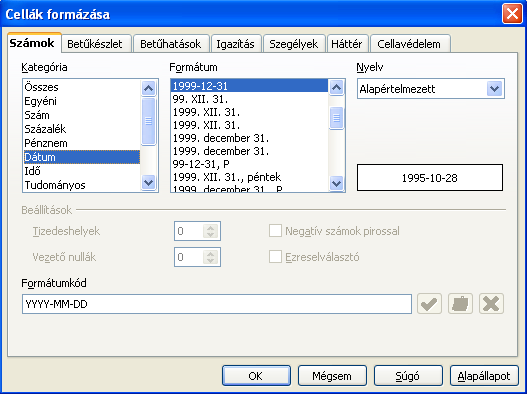
\includegraphics[width=13.944cm]{oocalcv1-img46.png}
\caption{Dátumformátumok}\label{Dátumformátumok}
\end{center}
\end{figure}

Minden számformátumot, így a dátumformátumot is
módosíthatjuk a \textbf{Formátum} menü \textbf{Cellák}
ablakában a \textbf{Számok} fület választva. \Aref{Dátumformátumok} ábrán
az A1 cella számformátumát látjuk, aminek tartalma 35000. A
\textbf{Dátum} kategóriát választva az
előnézetmezőben láthatjuk, hogy ennek a  számnak az
1995-10-28 dátum felel meg alapértelmezett dátumformátum
esetén. A \textbf{Formátumkód} ebben az esetben YYYY-MM-DD.

A Formátumkódot szerkeszthetjük is, a fenti példából is
látjuk, hogy négy Y betű az évszámot jeleníti meg. A
dátumformátum gyakran használt formátumkódjait \aref{DátumFormátumkódjai}
ábrán láthatjuk.

\begin{figure}[!h]
\begin{center}
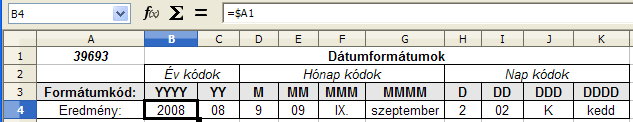
\includegraphics[width=15.999cm]{oocalcv1-img47.png}
\caption{Dátumformátumok formátumkódjai}\label{DátumFormátumkódjai}
\end{center}
\end{figure}

A B4 cella tartalma =\$A1, és ezt másoljuk a K4 celláig. Tehát a
B4:K4 tartomány minden cellája az A1 tartalmát mutatja. Ezeken a
cellákon a fölöttük látható dátumformátum van
beállítva.

Egyéni dátumformátumok használatára látunk három
példát \aref{EgyediDátumformátumok} ábrán.

\begin{figure}[!h]
\begin{center}
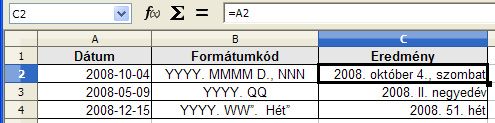
\includegraphics[width=13.095cm]{oocalcv1-img48.png}
\caption{Egyedi dátumformátumok}\label{EgyediDátumformátumok}
\end{center}
\end{figure}

A formátumkódot kiegészíthetjük tetszőleges szöveggel
is, ilyenkor a szöveget aposztrófjelek
(''...'') közé kell zárni.

Mind a dátumformátumot, mind a százalék- és
pénznemformátumot a Calc beíráskor automatikusan alkalmazza.
Ilyenkor a cella --  mint számok beírásakor --  jobbra igazított
lesz. Írjuk három cellába a következő tartalmakat: 2000Ft,
15\%, 2008.08.01. Figyeljük meg, hogy a Calc automatikusan alkalmazza
a pénznem, százalék és a dátum formátumokat. A cellák
tartalma pedig 2000, 0,15 és 39661 lesz, amit ellenőrizhetünk a
\textbf{Formátum} eszköztár \textbf{Számformátum:
Általános} parancsát alkalmazva.

A Calcban időértéket a szám tizedesjel utáni része
határozza meg.

Írjuk a 39700,5 számot egy cellába és válasszuk \aref{Időformátumok}
ábrán látható dátumformátumot. Látjuk,  hogy
esetünkben a 0,5 szám tizenkét óra nulla perc nulla
másodpercnek felel meg.

\begin{figure}[!h]
\begin{center}
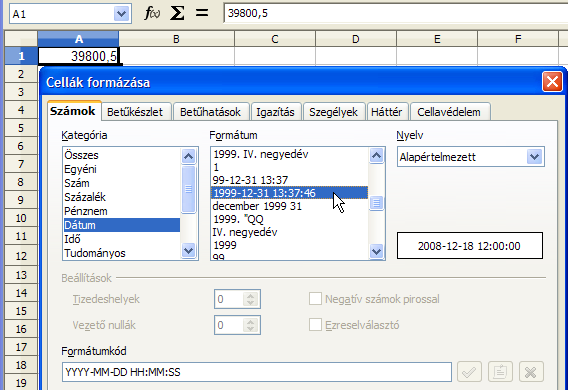
\includegraphics[width=15.027cm]{oocalcv1-img49.png}
\caption{Időformátumok}\label{Időformátumok}
\end{center}
\end{figure}
Megadhatunk dátum nélküli időértéket is,
értelemszerűen ilyenkor a szám egész része nulla lesz.

\Aref{Időformátumok} ábrán látjuk, hogy az előnézetmezőben látható
időformátumnak (12:00:00) a HH:MM:SS formátumkód felel meg.
További dátum- és időformátumokat \aref{TovábbiIdőformátumok} ábrán
találunk.

\begin{figure}[!h]
\begin{center}
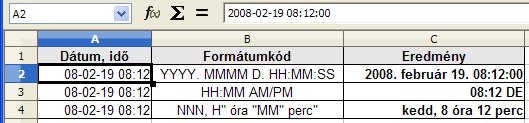
\includegraphics[width=13.995cm]{oocalcv1-img50.png}
\caption{További időformátumok}\label{TovábbiIdőformátumok}
\end{center}
\end{figure}

\clearpage
\section{Számformátumkódok}

Egyedi számformátumkódok használatával meghatározhatjuk,
hogy milyen formában jelenjenek meg a beírt számok a cellákban.
Legfeljebb három, egymástól pontosvesszővel elválasztott
formátumkódot határozhatunk meg egy cellára. Az első rész
a pozitív értékekre, a második a negatívokra és a harmadik
a nullára fog vonatkozni. Akár feltételeket is megadhatunk a
három részhez, a formátumkódok csak a feltételek
teljesülésekor hatnak.

Számok jelölésére a nullát (0) vagy a kettős keresztet
(\#) használhatjuk helykitöltőként
számformátumkódokban. A \# csak a lényeges számjegyeket
jeleníti meg, míg a 0, nullákat jelenít meg, ha a kód több
jegyből áll mint a beírt szám. Néhány
számformátumkódot egyszerűen beállíthatunk a
\textbf{Szám} kategóriában (\ref{SzámFormátumkódok} ábra).

\begin{figure}[!h]
\begin{center}
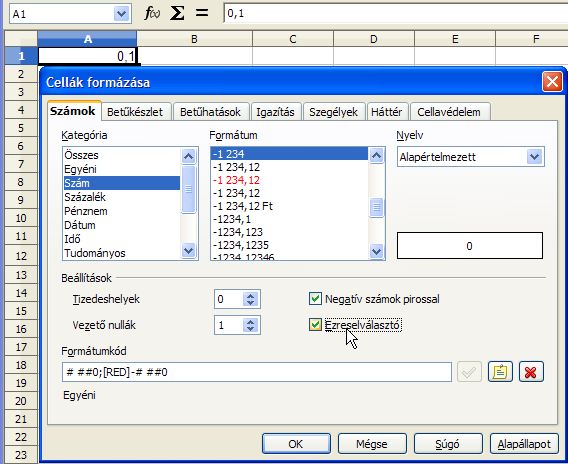
\includegraphics[width=15.027cm]{oocalcv1-img51.png}
\caption{Szám formátumkódok}\label{SzámFormátumkódok}
\end{center}
\end{figure}

Léptetőnyilak segítségével módosíthatjuk a tizedeshelyek
és a vezető nullák számát. Az \textbf{Ezreselválasztó}
bekapcsolása a \#\#\# kódrészletet hozza létre, ami ezres
csoportokba rendezi a szám egész részét. A \textbf{Negatív
számok pirossal} kapcsoló a pontosvessző, színkód [RED]
és a mínusz jel után megismétli a számformátumot. Negatív
számot írva a cellába az piros színű lesz, ezres
csoportosítású, két tizedes számjegyre kerekítve.
Kettőnél kevesebb tizedes számjegy esetén, azokat nullával
helyettesíti.

Kérdőjel (?) felhasználásával létrehozhatunk
formátumkódot, ami tört alakban jeleníti meg a számot a
cellában. A \#?/? formátumkód és 2,5 cellatartalom esetén a
cellában a következő kifejezést fogjuk látni: 2~$1/2$.

A tudományos számformátum segítségével nagyon nagy, vagy
nagyon kicsi számok tömör megjelenítését valósíthatjuk
meg. 200000000 (kétszázmillió) leírható
2*10\textsuperscript{8} módon is, amit a Calc a
következőképpen jelenít meg: 2,00E+8. A formátumkód ebben
az esetben: 0,00E+\#.

A következő formátumkód négy részből áll, a negyedik
akkor fog végrehajtódni, ha a cellába nem számot írunk. Ez
hasznos lehet, hiszen figyelmezteti a felhasználót, ha az
például a 0 számjegy helyett O betűt ír:\\
{\sffamily\bfseries
[MAGENTA]\#\#\#0"db";[RED]-\#\#\#0"db";[GREEN]\#\#\#0"db";"Ön nem számot írt!"}.

Tehát a formátumkód, pozitív számot beírva, azt ezres
csoportosítással egészre kerekítve, magenta színnel
jeleníti meg, a szám után szóköz és
''db'' karakterekkel. Negatív
szám és nulla beírása esetén a kódban megadott színnel
jelennek meg a számok, a többi formátum ugyanaz mint pozitív
számnál. Szöveg beírásakor (pl. 5OO) a következő
figyelmeztető üzenet jelenik meg: ,,Ön nem
számot írt!'' Érdekes, hogy a kerekítés
miatt az is előfordulhat, hogy három különböző
színű ,,0 db''-t látunk a
cellában. Ilyen számok pl. a -0,2; 0 és 0,2. Mindhárom szám
egészre kerekítve a cellában ,,0~db''-ként jelenik meg,
de a színük magenta, piros és zöld.

A Calcban a következő színkódokat használhatjuk: CYAN
(cián), BLACK (fekete), MAGENTA (magenta), WHITE (fehér), GREEN
(zöld), BLUE (kék), RED (piros) és YELLOW (sárga).

Meghatározhatunk olyan számformátumot, ami csak bizonyos
feltétel esetén teljesül. A feltételekben számokat és
matematikai operátorokat használhatunk. A Calc súgójában a
következő példát találjuk a feltételes
számformátumra:


{\sffamily\bfseries
[BLUE][<0]\#,0"${}^\circ$C";[RED][>=30]\#,0"${}^\circ$C";[BLACK]\#,0"${}^\circ$C"}.

Ezt a formátumot alkalmazva egy cellára, a beírt negatív szám
kék színű lesz, 0 és 30 fok között fekete, 30 és
annál nagyobb pedig piros. Mindhárom esetben a számok után
megjelenik a ,,$^\circ$C'' kifejezés.

